\documentclass{article}

\usepackage[margin=1in]{geometry}

\usepackage{graphicx}

\title{Report}

\begin{document}

\maketitle

Result of MMPBSA calculations on a congeneric intercalator series interacting with a ds-DNA from a crystal structure (1Z3F). After a more careful analysis I was able to show a separation between the two ligand types (3 vs 4 membered intercalator), but in more general the correlation to experiment needs some improvement. 

\begin{figure}
  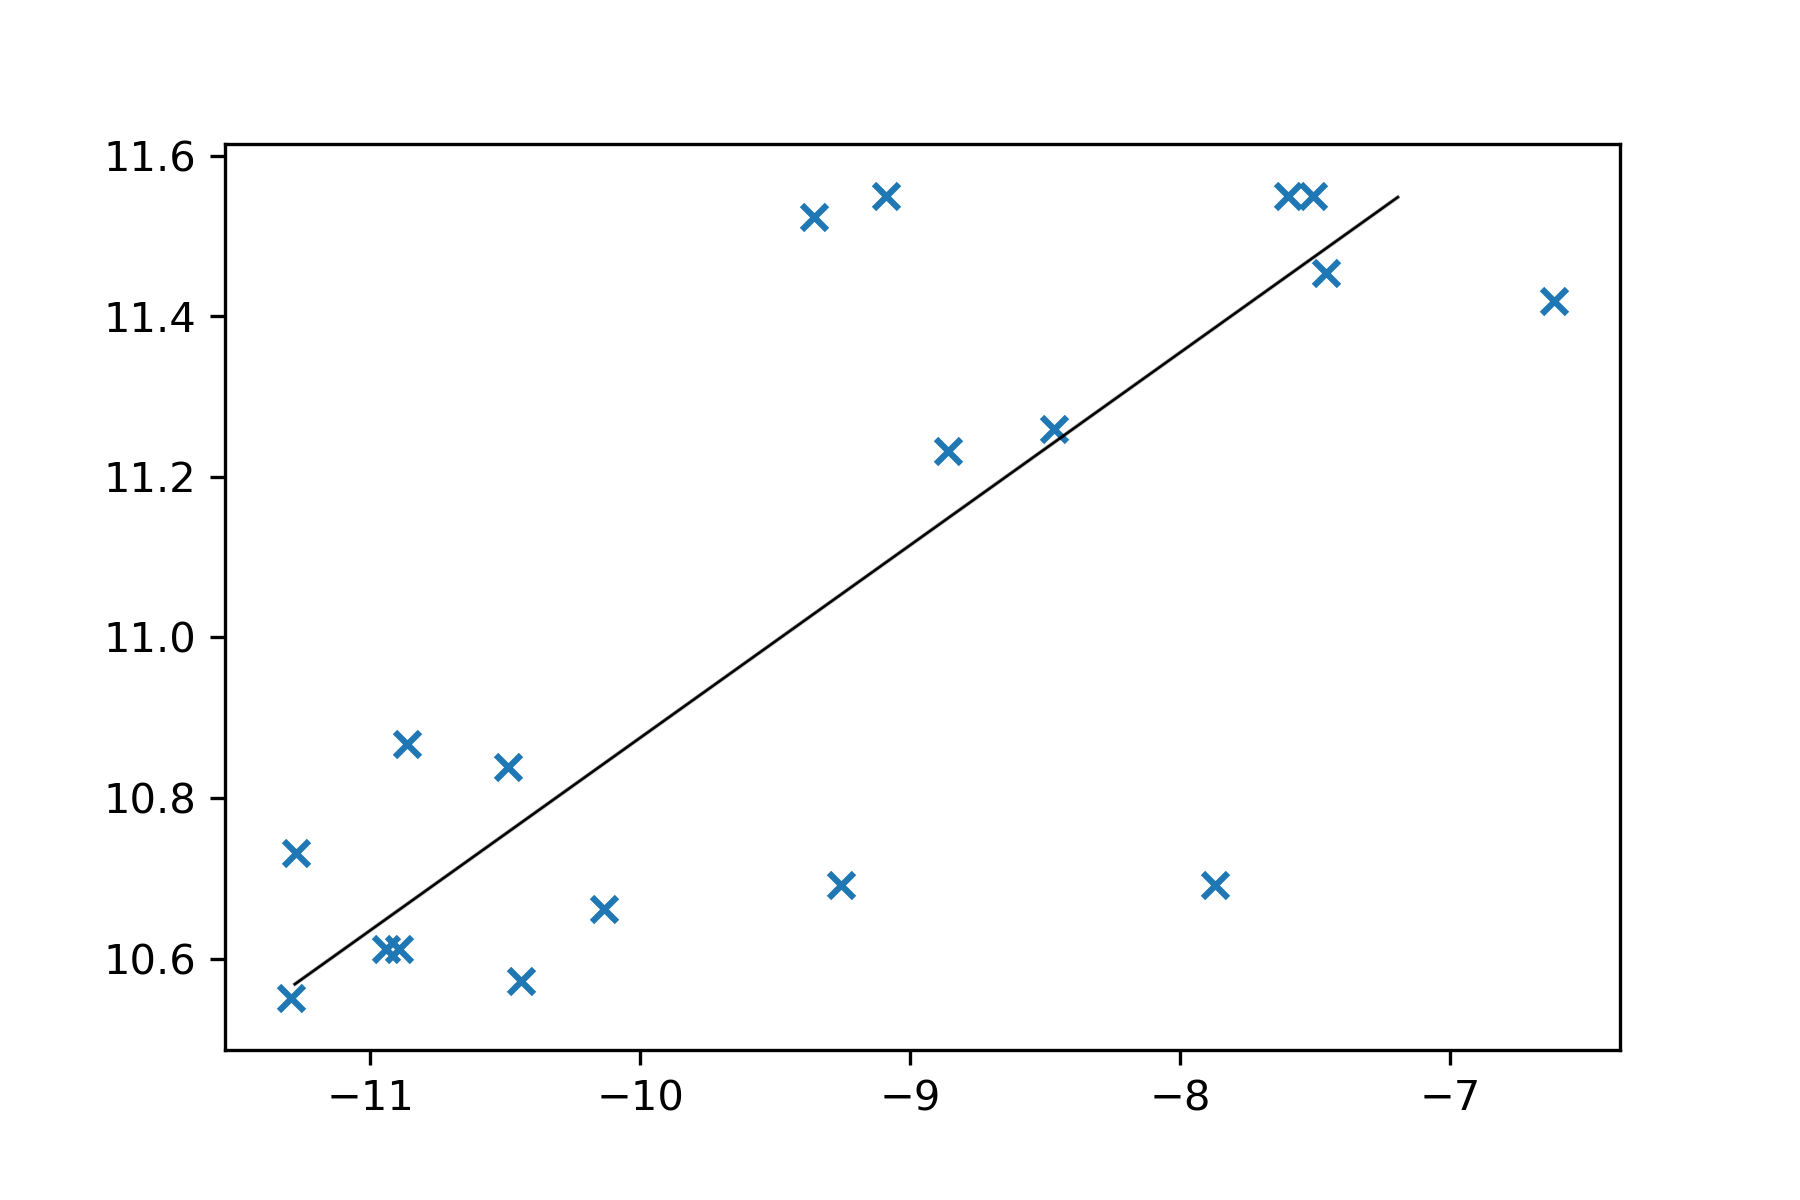
\includegraphics{res-vs-exp}
  \caption{A plot of the results versus experimental values. There is a correlation but a number of outliers worsen the overall result.}
  \label{fig1}
\end{figure}  

\begin{figure}
  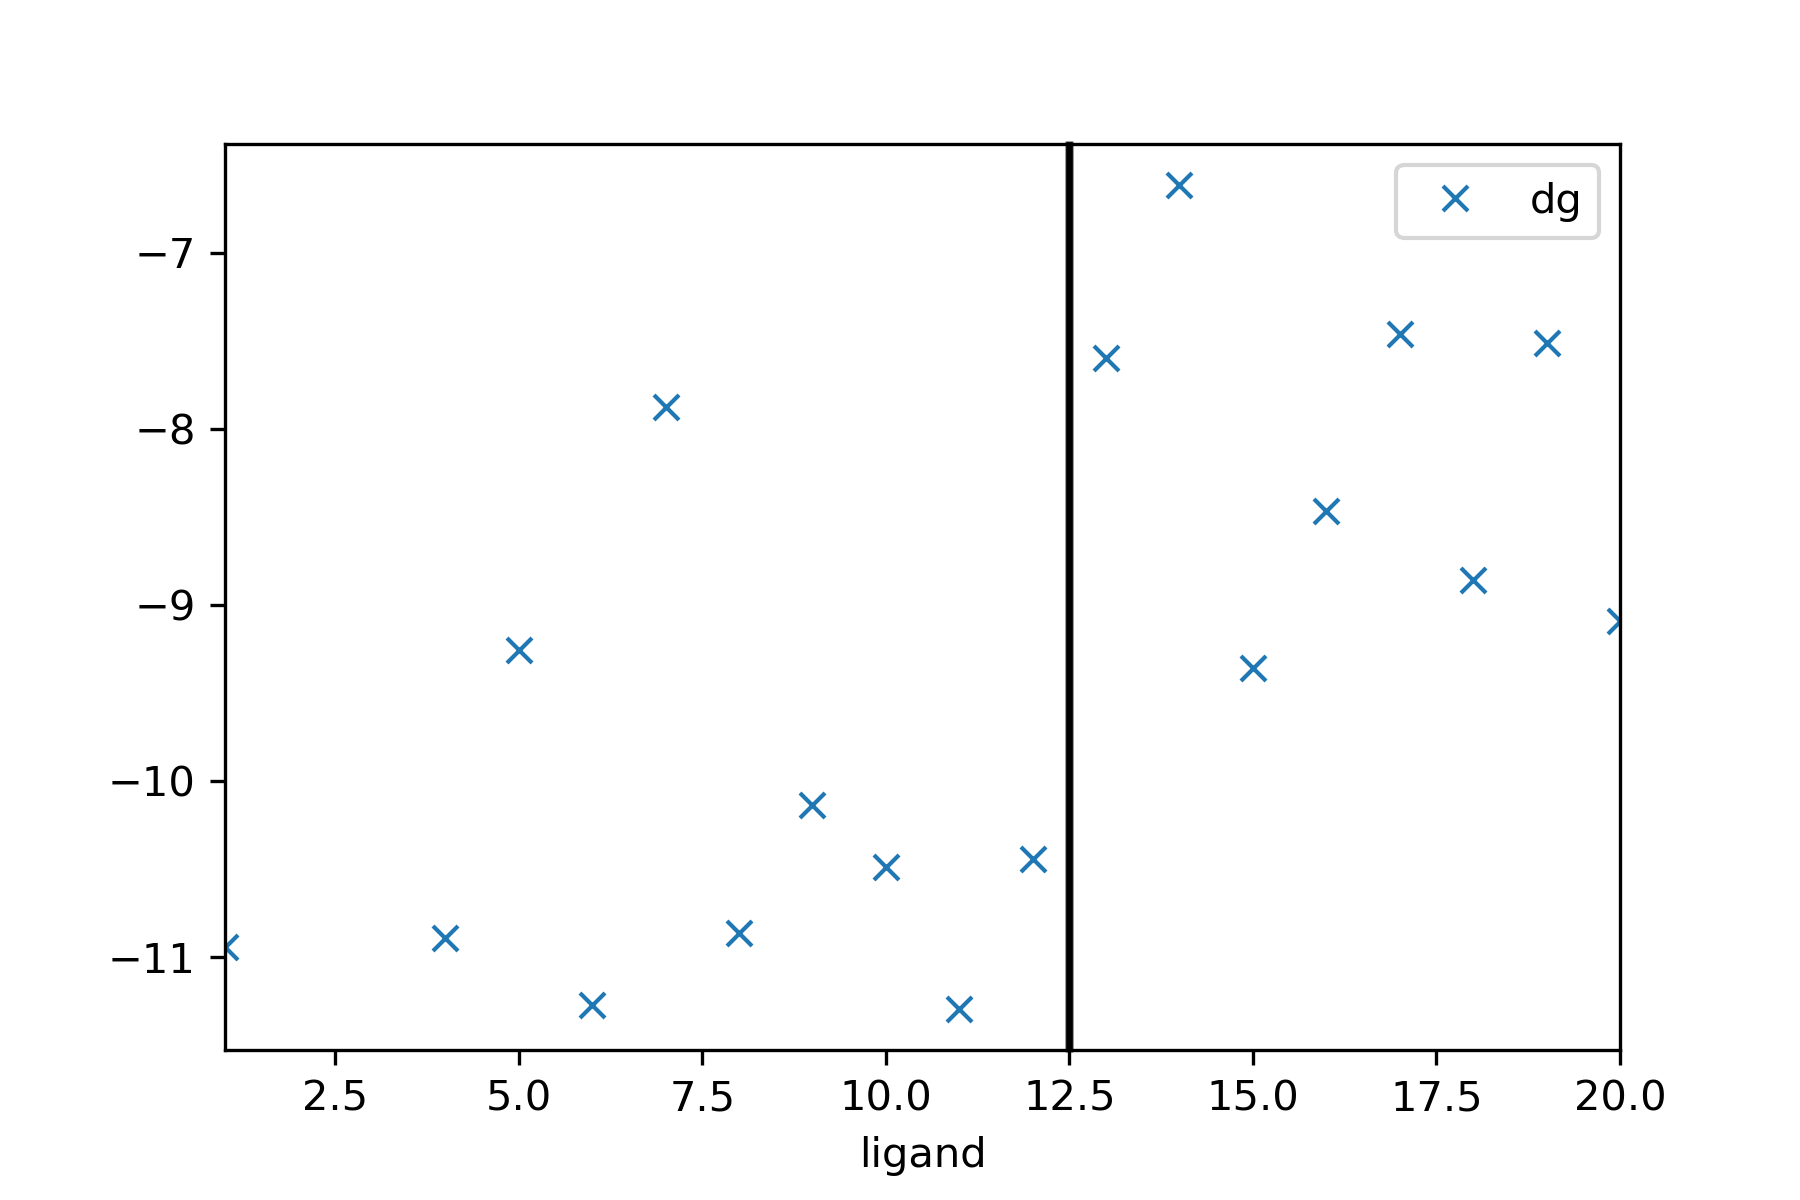
\includegraphics{fig}
  \caption{A plot of the dG values for each ligand. You can clearly see the difference between the 3 and 4 membered intercalator (black line), and a clustering inside the groups.}
  \label{fi2}
\end{figure}
  
\end{document}